\begin{figure}[]\centering
  \definecolor{aa}{RGB}{227,26,28}
\definecolor{ab}{RGB}{56,125,184}
\definecolor{ac}{RGB}{77,176,74}
\definecolor{ak}{RGB}{0,0,0}

% GNUPLOT: LaTeX picture with Postscript
\begingroup
  \makeatletter
  \providecommand\color[2][]{%
    \GenericError{(gnuplot) \space\space\space\@spaces}{%
      Package color not loaded in conjunction with
      terminal option `colourtext'%
    }{See the gnuplot documentation for explanation.%
    }{Either use 'blacktext' in gnuplot or load the package
      color.sty in LaTeX.}%
    \renewcommand\color[2][]{}%
  }%
  \providecommand\includegraphics[2][]{%
    \GenericError{(gnuplot) \space\space\space\@spaces}{%
      Package graphicx or graphics not loaded%
    }{See the gnuplot documentation for explanation.%
    }{The gnuplot epslatex terminal needs graphicx.sty or graphics.sty.}%
    \renewcommand\includegraphics[2][]{}%
  }%
  \providecommand\rotatebox[2]{#2}%
  \@ifundefined{ifGPcolor}{%
    \newif\ifGPcolor
    \GPcolorfalse
  }{}%
  \@ifundefined{ifGPblacktext}{%
    \newif\ifGPblacktext
    \GPblacktexttrue
  }{}%
  % define a \g@addto@macro without @ in the name:
  \let\gplgaddtomacro\g@addto@macro
  % define empty templates for all commands taking text:
  \gdef\gplfronttext{}%
  \gdef\gplfronttext{}%
  \makeatother
  \ifGPblacktext
    % no textcolor at all
    \def\colorrgb#1{}%
    \def\colorgray#1{}%
  \else
    % gray or color?
    \ifGPcolor
      \def\colorrgb#1{\color[rgb]{#1}}%
      \def\colorgray#1{\color[gray]{#1}}%
      \expandafter\def\csname LTw\endcsname{\color{white}}%
      \expandafter\def\csname LTb\endcsname{\color{black}}%
      \expandafter\def\csname LTa\endcsname{\color{black}}%
      \expandafter\def\csname LT0\endcsname{\color[rgb]{1,0,0}}%
      \expandafter\def\csname LT1\endcsname{\color[rgb]{0,1,0}}%
      \expandafter\def\csname LT2\endcsname{\color[rgb]{0,0,1}}%
      \expandafter\def\csname LT3\endcsname{\color[rgb]{1,0,1}}%
      \expandafter\def\csname LT4\endcsname{\color[rgb]{0,1,1}}%
      \expandafter\def\csname LT5\endcsname{\color[rgb]{1,1,0}}%
      \expandafter\def\csname LT6\endcsname{\color[rgb]{0,0,0}}%
      \expandafter\def\csname LT7\endcsname{\color[rgb]{1,0.3,0}}%
      \expandafter\def\csname LT8\endcsname{\color[rgb]{0.5,0.5,0.5}}%
    \else
      % gray
      \def\colorrgb#1{\color{black}}%
      \def\colorgray#1{\color[gray]{#1}}%
      \expandafter\def\csname LTw\endcsname{\color{white}}%
      \expandafter\def\csname LTb\endcsname{\color{black}}%
      \expandafter\def\csname LTa\endcsname{\color{black}}%
      \expandafter\def\csname LT0\endcsname{\color{black}}%
      \expandafter\def\csname LT1\endcsname{\color{black}}%
      \expandafter\def\csname LT2\endcsname{\color{black}}%
      \expandafter\def\csname LT3\endcsname{\color{black}}%
      \expandafter\def\csname LT4\endcsname{\color{black}}%
      \expandafter\def\csname LT5\endcsname{\color{black}}%
      \expandafter\def\csname LT6\endcsname{\color{black}}%
      \expandafter\def\csname LT7\endcsname{\color{black}}%
      \expandafter\def\csname LT8\endcsname{\color{black}}%
    \fi
  \fi
    \setlength{\unitlength}{0.0500bp}%
    \ifx\gptboxheight\undefined%
      \newlength{\gptboxheight}%
      \newlength{\gptboxwidth}%
      \newsavebox{\gptboxtext}%
    \fi%
    \setlength{\fboxrule}{0.5pt}%
    \setlength{\fboxsep}{1pt}%
\begin{picture}(5000.00,5000.00)%
    \gplgaddtomacro\gplfronttext{%
      \colorrgb{0.15,0.15,0.15}%
      \put(391,1564){\makebox(0,0)[r]{\strut{}$6.0$}}%
      \colorrgb{0.15,0.15,0.15}%
      \put(391,1988){\makebox(0,0)[r]{\strut{}$8.0$}}%
      \colorrgb{0.15,0.15,0.15}%
      \put(391,2413){\makebox(0,0)[r]{\strut{}$10.0$}}%
      \colorrgb{0.15,0.15,0.15}%
      \put(391,2837){\makebox(0,0)[r]{\strut{}$12.0$}}%
      \colorrgb{0.15,0.15,0.15}%
      \put(391,3262){\makebox(0,0)[r]{\strut{}$14.0$}}%
      \colorrgb{0.15,0.15,0.15}%
      \put(391,3687){\makebox(0,0)[r]{\strut{}$16.0$}}%
      \colorrgb{0.00,0.00,0.00}%
      \put(672,1280){\makebox(0,0){\strut{}$-2.0$}}%
      \colorrgb{0.00,0.00,0.00}%
      \put(1096,1280){\makebox(0,0){\strut{}$0.0$}}%
      \colorrgb{0.00,0.00,0.00}%
      \put(1521,1280){\makebox(0,0){\strut{}$2.0$}}%
      \colorrgb{0.00,0.00,0.00}%
      \put(1945,1280){\makebox(0,0){\strut{}$4.0$}}%
      \colorrgb{0.00,0.00,0.00}%
      \put(2370,1280){\makebox(0,0){\strut{}$6.0$}}%

      \put(1020,4104){\makebox(0,0){\strut{}{\color{ak}{\rule[0.6mm]{0.5cm}{0.5mm}}} \small Τροχιά αισθητήρα}}
      \put(2570,4104){\makebox(0,0){\strut{}{\color{aa}{\rule[0.6mm]{0.5cm}{0.5mm}}} \small PLICP}}
      \put(3500,4104){\makebox(0,0){\strut{}{\color{ab}{\rule[0.6mm]{0.5cm}{0.5mm}}} \small NDT}}
      \put(4440,4104){\makebox(0,0){\strut{}{\color{ac}{\rule[0.6mm]{0.5cm}{0.5mm}}} \small \texttt{fsm}}}
      \put(1500,1004){\makebox(0,0){\strut{} \small Πυκνές μετρήσεις}}
      \put(3600,1004){\makebox(0,0){\strut{} \small Αραιές μετρήσεις}}
    }%
    \gplgaddtomacro\gplfronttext{%
    }%
    \gplgaddtomacro\gplfronttext{%
      \colorrgb{0.00,0.00,0.00}%
      \put(2822,1280){\makebox(0,0){\strut{}$-2.0$}}%
      \colorrgb{0.00,0.00,0.00}%
      \put(3246,1280){\makebox(0,0){\strut{}$0.0$}}%
      \colorrgb{0.00,0.00,0.00}%
      \put(3671,1280){\makebox(0,0){\strut{}$2.0$}}%
      \colorrgb{0.00,0.00,0.00}%
      \put(4095,1280){\makebox(0,0){\strut{}$4.0$}}%
      \colorrgb{0.00,0.00,0.00}%
      \put(4520,1280){\makebox(0,0){\strut{}$6.0$}}%
    }%
    \gplgaddtomacro\gplfronttext{%
    }%
    \put(0,0){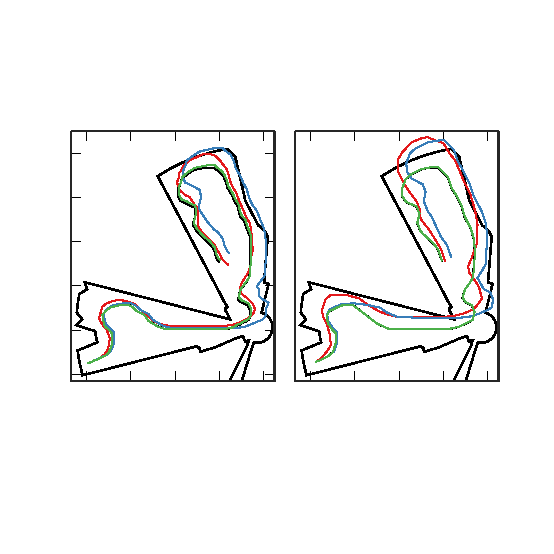
\includegraphics{./figures/parts/02/chapters/05/sections/04/odom_test_5_vs_6}}%
    \gplfronttext
  \end{picture}%
\endgroup

  \vspace{-2cm}
  \caption{\small Scan-matching as ``laser odometry": the robot moves from the
           lower left portion of the environment to the upper right, capturing
           2D range scans along its trajectory. The coloured routes show the
           estimated path of the robot derived from each method. The proposed
           method's error is invariant to angular and locational displacement}
  \label{}
\end{figure}

\begin{figure}[]\centering
  \definecolor{pp}{RGB}{127,201,127}
\definecolor{cc}{RGB}{0,0,0}
\definecolor{oo}{RGB}{251,128,114}

% GNUPLOT: LaTeX picture with Postscript
\begingroup
  \makeatletter
  \providecommand\color[2][]{%
    \GenericError{(gnuplot) \space\space\space\@spaces}{%
      Package color not loaded in conjunction with
      terminal option `colourtext'%
    }{See the gnuplot documentation for explanation.%
    }{Either use 'blacktext' in gnuplot or load the package
      color.sty in LaTeX.}%
    \renewcommand\color[2][]{}%
  }%
  \providecommand\includegraphics[2][]{%
    \GenericError{(gnuplot) \space\space\space\@spaces}{%
      Package graphicx or graphics not loaded%
    }{See the gnuplot documentation for explanation.%
    }{The gnuplot epslatex terminal needs graphicx.sty or graphics.sty.}%
    \renewcommand\includegraphics[2][]{}%
  }%
  \providecommand\rotatebox[2]{#2}%
  \@ifundefined{ifGPcolor}{%
    \newif\ifGPcolor
    \GPcolorfalse
  }{}%
  \@ifundefined{ifGPblacktext}{%
    \newif\ifGPblacktext
    \GPblacktexttrue
  }{}%
  % define a \g@addto@macro without @ in the name:
  \let\gplgaddtomacro\g@addto@macro
  % define empty templates for all commands taking text:
  \gdef\gplfronttext{}%
  \gdef\gplfronttext{}%
  \makeatother
  \ifGPblacktext
    % no textcolor at all
    \def\colorrgb#1{}%
    \def\colorgray#1{}%
  \else
    % gray or color?
    \ifGPcolor
      \def\colorrgb#1{\color[rgb]{#1}}%
      \def\colorgray#1{\color[gray]{#1}}%
      \expandafter\def\csname LTw\endcsname{\color{white}}%
      \expandafter\def\csname LTb\endcsname{\color{black}}%
      \expandafter\def\csname LTa\endcsname{\color{black}}%
      \expandafter\def\csname LT0\endcsname{\color[rgb]{1,0,0}}%
      \expandafter\def\csname LT1\endcsname{\color[rgb]{0,1,0}}%
      \expandafter\def\csname LT2\endcsname{\color[rgb]{0,0,1}}%
      \expandafter\def\csname LT3\endcsname{\color[rgb]{1,0,1}}%
      \expandafter\def\csname LT4\endcsname{\color[rgb]{0,1,1}}%
      \expandafter\def\csname LT5\endcsname{\color[rgb]{1,1,0}}%
      \expandafter\def\csname LT6\endcsname{\color[rgb]{0,0,0}}%
      \expandafter\def\csname LT7\endcsname{\color[rgb]{1,0.3,0}}%
      \expandafter\def\csname LT8\endcsname{\color[rgb]{0.5,0.5,0.5}}%
    \else
      % gray
      \def\colorrgb#1{\color{black}}%
      \def\colorgray#1{\color[gray]{#1}}%
      \expandafter\def\csname LTw\endcsname{\color{white}}%
      \expandafter\def\csname LTb\endcsname{\color{black}}%
      \expandafter\def\csname LTa\endcsname{\color{black}}%
      \expandafter\def\csname LT0\endcsname{\color{black}}%
      \expandafter\def\csname LT1\endcsname{\color{black}}%
      \expandafter\def\csname LT2\endcsname{\color{black}}%
      \expandafter\def\csname LT3\endcsname{\color{black}}%
      \expandafter\def\csname LT4\endcsname{\color{black}}%
      \expandafter\def\csname LT5\endcsname{\color{black}}%
      \expandafter\def\csname LT6\endcsname{\color{black}}%
      \expandafter\def\csname LT7\endcsname{\color{black}}%
      \expandafter\def\csname LT8\endcsname{\color{black}}%
    \fi
  \fi
    \setlength{\unitlength}{0.0500bp}%
    \ifx\gptboxheight\undefined%
      \newlength{\gptboxheight}%
      \newlength{\gptboxwidth}%
      \newsavebox{\gptboxtext}%
    \fi%
    \setlength{\fboxrule}{0.5pt}%
    \setlength{\fboxsep}{1pt}%
\begin{picture}(8000.00,8000.00)%
    \gplgaddtomacro\gplfronttext{%
    }%
    \gplgaddtomacro\gplfronttext{%
      \colorrgb{0.00,0.00,0.00}%
      \put(3999,7959){\makebox(0,0){\strut{}\small Αρχική συνθήκη}}%
      \put(600, 3770){\makebox(0,0){\strut{}{\color{pp}{\rule[0.6mm]{0.5cm}{0.5mm}}} \small Σφάλμα θέσης [m]}}
      \put(3420,3770){\makebox(0,0){\strut{}{\color{oo}{\rule[0.6mm]{0.5cm}{0.5mm}}} \small Σφάλμα προσανατολισμού [rad]}}
      \put(7020,3770){\makebox(0,0){\strut{}{\color{cc}{\rule[0.6mm]{0.5cm}{0.5mm}}} \small Οικεία εσωτερική μετρική σφάλματος [m]}}
    }%
    \gplgaddtomacro\gplfronttext{%
    }%
    \gplgaddtomacro\gplfronttext{%
      \colorrgb{0.00,0.00,0.00}%
      \put(1839,5959){\makebox(0,0){\strut{}\small Εξέλιξη ευθυγράμμισης FastGICP}}%
    }%
    \gplgaddtomacro\gplfronttext{%
    }%
    \gplgaddtomacro\gplfronttext{%
      \colorrgb{0.00,0.00,0.00}%
      \put(6159,5959){\makebox(0,0){\strut{}\small Εξέλιξη ευθυγράμμισης \texttt{fsm}}}%
    }%
    \gplgaddtomacro\gplfronttext{%
      \colorrgb{0.00,0.45,0.74}%
      \put(508,2400){\makebox(0,0)[r]{\strut{}\scriptsize $0.0$}}%
      \colorrgb{0.00,0.45,0.74}%
      \put(508,2543){\makebox(0,0)[r]{\strut{}\scriptsize $0.2$}}%
      \colorrgb{0.00,0.45,0.74}%
      \put(508,2685){\makebox(0,0)[r]{\strut{}\scriptsize $0.4$}}%
      \colorrgb{0.00,0.45,0.74}%
      \put(508,2828){\makebox(0,0)[r]{\strut{}\scriptsize $0.6$}}%
      \colorrgb{0.00,0.45,0.74}%
      \put(508,2971){\makebox(0,0)[r]{\strut{}\scriptsize $0.8$}}%
      \colorrgb{0.00,0.45,0.74}%
      \put(508,3114){\makebox(0,0)[r]{\strut{}\scriptsize $1.0$}}%
      \colorrgb{0.00,0.45,0.74}%
      \put(508,3256){\makebox(0,0)[r]{\strut{}\scriptsize $1.2$}}%
      \colorrgb{0.00,0.45,0.74}%
      \put(508,3399){\makebox(0,0)[r]{\strut{}\scriptsize $1.4$}}%
    }%
    \gplgaddtomacro\gplfronttext{%
    }%
    \gplgaddtomacro\gplfronttext{%
      \colorrgb{0.15,0.15,0.15}%
      \put(640,2180){\makebox(0,0){\strut{}\scriptsize $0$}}%
      \colorrgb{0.15,0.15,0.15}%
      \put(1089,2180){\makebox(0,0){\strut{}\scriptsize $10$}}%
      \colorrgb{0.15,0.15,0.15}%
      \put(1538,2180){\makebox(0,0){\strut{}\scriptsize $20$}}%
      \colorrgb{0.85,0.33,0.10}%
      \put(1715,2400){\makebox(0,0)[l]{\strut{}}}%
      \colorrgb{0.85,0.33,0.10}%
      \put(1715,2600){\makebox(0,0)[l]{\strut{}}}%
      \colorrgb{0.85,0.33,0.10}%
      \put(1715,2800){\makebox(0,0)[l]{\strut{}}}%
      \colorrgb{0.85,0.33,0.10}%
      \put(1715,2999){\makebox(0,0)[l]{\strut{}}}%
      \colorrgb{0.85,0.33,0.10}%
      \put(1715,3199){\makebox(0,0)[l]{\strut{}}}%
      \colorrgb{0.85,0.33,0.10}%
      \put(1715,3399){\makebox(0,0)[l]{\strut{}}}%
    }%
    \gplgaddtomacro\gplfronttext{%
    }%
    \gplgaddtomacro\gplfronttext{%
      \colorrgb{1.00,0.00,1.00}%
      \put(2108,2400){\makebox(0,0)[r]{\strut{}\scriptsize $0$}}%
      \colorrgb{1.00,0.00,1.00}%
      \put(2108,2574){\makebox(0,0)[r]{\strut{}\scriptsize $0.18$}}%
      \colorrgb{1.00,0.00,1.00}%
      \put(2108,2749){\makebox(0,0)[r]{\strut{}\scriptsize $0.35$}}%
      \colorrgb{1.00,0.00,1.00}%
      \put(2108,2923){\makebox(0,0)[r]{\strut{}\scriptsize $0.52$}}%
      \colorrgb{1.00,0.00,1.00}%
      \put(2108,3097){\makebox(0,0)[r]{\strut{}\scriptsize $0.70$}}%
      \colorrgb{1.00,0.00,1.00}%
      \put(2108,3272){\makebox(0,0)[r]{\strut{}\scriptsize $0.87$}}%
    }%
    \gplgaddtomacro\gplfronttext{%
    }%
    \gplgaddtomacro\gplfronttext{%
      \colorrgb{0.15,0.15,0.15}%
      \put(2240,2180){\makebox(0,0){\strut{}\scriptsize $0$}}%
      \colorrgb{0.15,0.15,0.15}%
      \put(2689,2180){\makebox(0,0){\strut{}\scriptsize $10$}}%
      \colorrgb{0.15,0.15,0.15}%
      \put(3138,2180){\makebox(0,0){\strut{}\scriptsize $20$}}%
      \colorrgb{0.85,0.33,0.10}%
      \put(3315,2400){\makebox(0,0)[l]{\strut{}\scriptsize $0$}}%
      \colorrgb{0.85,0.33,0.10}%
      \put(3315,2600){\makebox(0,0)[l]{\strut{}\scriptsize $100$}}%
      \colorrgb{0.85,0.33,0.10}%
      \put(3315,2800){\makebox(0,0)[l]{\strut{}\scriptsize $200$}}%
      \colorrgb{0.85,0.33,0.10}%
      \put(3315,2999){\makebox(0,0)[l]{\strut{}\scriptsize $300$}}%
      \colorrgb{0.85,0.33,0.10}%
      \put(3315,3199){\makebox(0,0)[l]{\strut{}\scriptsize $400$}}%
      \colorrgb{0.85,0.33,0.10}%
      \put(3315,3399){\makebox(0,0)[l]{\strut{}\scriptsize $500$}}%
    }%
    \gplgaddtomacro\gplfronttext{%
    }%
    \gplgaddtomacro\gplfronttext{%
      \colorrgb{0.00,0.45,0.74}%
      \put(4668,2400){\makebox(0,0)[r]{\strut{}\scriptsize $0.0$}}%
      \colorrgb{0.00,0.45,0.74}%
      \put(4668,2650){\makebox(0,0)[r]{\strut{}\scriptsize $0.1$}}%
      \colorrgb{0.00,0.45,0.74}%
      \put(4668,2900){\makebox(0,0)[r]{\strut{}\scriptsize $0.2$}}%
      \colorrgb{0.00,0.45,0.74}%
      \put(4668,3149){\makebox(0,0)[r]{\strut{}\scriptsize $0.3$}}%
      \colorrgb{0.00,0.45,0.74}%
      \put(4668,3399){\makebox(0,0)[r]{\strut{}\scriptsize $0.4$}}%
    }%
    \gplgaddtomacro\gplfronttext{%
    }%
    \gplgaddtomacro\gplfronttext{%
      \colorrgb{0.15,0.15,0.15}%
      \put(5010,2180){\makebox(0,0){\strut{}\scriptsize $2$}}%
      \colorrgb{0.15,0.15,0.15}%
      \put(5219,2180){\makebox(0,0){\strut{}\scriptsize $4$}}%
      \colorrgb{0.15,0.15,0.15}%
      \put(5429,2180){\makebox(0,0){\strut{}\scriptsize $6$}}%
      \colorrgb{0.15,0.15,0.15}%
      \put(5638,2180){\makebox(0,0){\strut{}\scriptsize $8$}}%
      \colorrgb{0.85,0.33,0.10}%
      \put(5875,2400){\makebox(0,0)[l]{\strut{}}}%
      \colorrgb{0.85,0.33,0.10}%
      \put(5875,2650){\makebox(0,0)[l]{\strut{}}}%
      \colorrgb{0.85,0.33,0.10}%
      \put(5875,2900){\makebox(0,0)[l]{\strut{}}}%
      \colorrgb{0.85,0.33,0.10}%
      \put(5875,3149){\makebox(0,0)[l]{\strut{}}}%
      \colorrgb{0.85,0.33,0.10}%
      \put(5875,3399){\makebox(0,0)[l]{\strut{}}}%
    }%
    \gplgaddtomacro\gplfronttext{%
    }%
    \gplgaddtomacro\gplfronttext{%
      \colorrgb{1.00,0.00,1.00}%
      \colorrgb{1.00,0.00,1.00}%
      \put(6268,2400){\makebox(0,0)[r]{\strut{}\scriptsize $0$}}%
      \colorrgb{1.00,0.00,1.00}%
      \put(6268,2574){\makebox(0,0)[r]{\strut{}\scriptsize $0.18$}}%
      \colorrgb{1.00,0.00,1.00}%
      \put(6268,2749){\makebox(0,0)[r]{\strut{}\scriptsize $0.35$}}%
      \colorrgb{1.00,0.00,1.00}%
      \put(6268,2923){\makebox(0,0)[r]{\strut{}\scriptsize $0.52$}}%
      \colorrgb{1.00,0.00,1.00}%
      \put(6268,3097){\makebox(0,0)[r]{\strut{}\scriptsize $0.70$}}%
      \colorrgb{1.00,0.00,1.00}%
      \put(6268,3272){\makebox(0,0)[r]{\strut{}\scriptsize $0.87$}}%
    }%
    \gplgaddtomacro\gplfronttext{%
    }%
    \gplgaddtomacro\gplfronttext{%
      \colorrgb{0.15,0.15,0.15}%
      \put(6610,2180){\makebox(0,0){\strut{}\scriptsize $2$}}%
      \colorrgb{0.15,0.15,0.15}%
      \put(6819,2180){\makebox(0,0){\strut{}\scriptsize $4$}}%
      \colorrgb{0.15,0.15,0.15}%
      \put(7029,2180){\makebox(0,0){\strut{}\scriptsize $6$}}%
      \colorrgb{0.15,0.15,0.15}%
      \put(7238,2180){\makebox(0,0){\strut{}\scriptsize $8$}}%
      \colorrgb{0.85,0.33,0.10}%
      \put(7475,2400){\makebox(0,0)[l]{\strut{}\scriptsize $0$}}%
      \colorrgb{0.85,0.33,0.10}%
      \put(7475,2650){\makebox(0,0)[l]{\strut{}\scriptsize $50$}}%
      \colorrgb{0.85,0.33,0.10}%
      \put(7475,2900){\makebox(0,0)[l]{\strut{}\scriptsize $100$}}%
      \colorrgb{0.85,0.33,0.10}%
      \put(7475,3149){\makebox(0,0)[l]{\strut{}\scriptsize $150$}}%
      \colorrgb{0.85,0.33,0.10}%
      \put(7475,3399){\makebox(0,0)[l]{\strut{}\scriptsize $200$}}%
    }%
    \gplgaddtomacro\gplfronttext{%
    }%
    \gplgaddtomacro\gplfronttext{%
    }%
    \gplgaddtomacro\gplfronttext{%
      \colorrgb{0.00,0.00,0.00}%
      \put(1839,1799){\makebox(0,0){\strut{}\small Τελική ευθυγράμμιση FastGICP}}%
    }%
    \gplgaddtomacro\gplfronttext{%
    }%
    \gplgaddtomacro\gplfronttext{%
      \colorrgb{0.00,0.00,0.00}%
      \put(6159,1799){\makebox(0,0){\strut{}\small Τελική ευθυγράμμιση \texttt{fsm}}}%
    }%
    \put(0,0){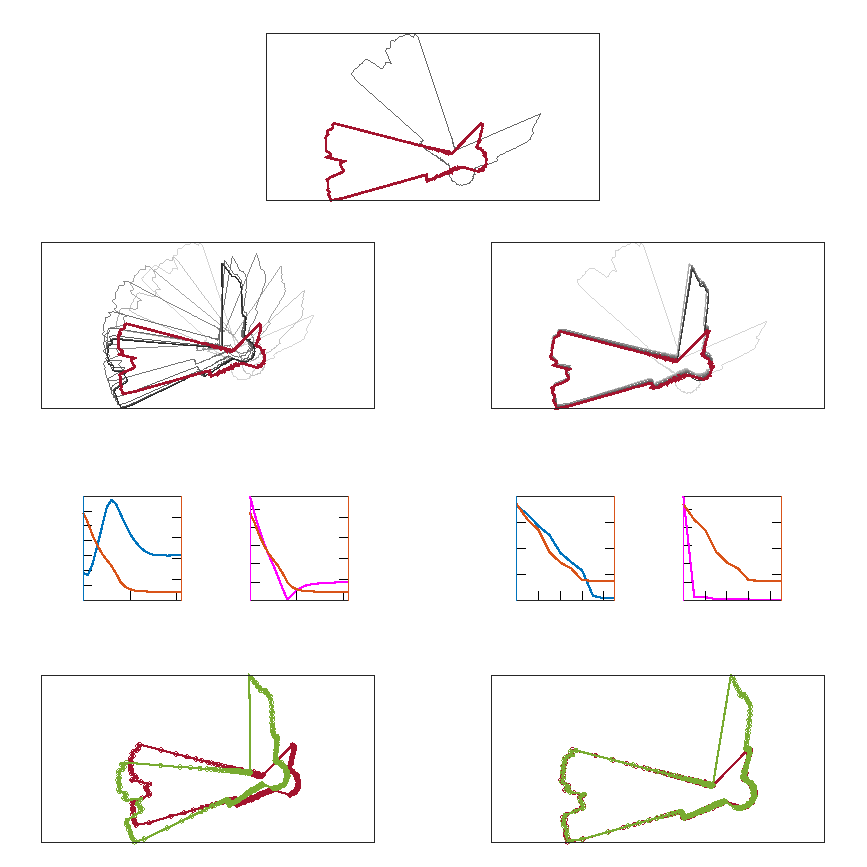
\includegraphics{./figures/parts/02/chapters/05/sections/04/fsm_vs_fgi}}%
    \gplfronttext
  \end{picture}%
\endgroup

  \caption{$\sigma_R = 0.03$, $\delta = (0.35, 0.1, -\pi/3)$. fsm: 0.0098 m, 0.08 deg.
  fgi: 0.61 m, 9.94 deg. up to 7.28 m/s, 720 deg/sec}
  \label{}
\end{figure}

\begin{figure}[]\centering
  \definecolor{aa}{rgb}{0.00000   0.44700   0.74100}
\definecolor{ac}{rgb}{1.00000   0.00000   1.00000}

% GNUPLOT: LaTeX picture with Postscript
\begingroup
  \makeatletter
  \providecommand\color[2][]{%
    \GenericError{(gnuplot) \space\space\space\@spaces}{%
      Package color not loaded in conjunction with
      terminal option `colourtext'%
    }{See the gnuplot documentation for explanation.%
    }{Either use 'blacktext' in gnuplot or load the package
      color.sty in LaTeX.}%
    \renewcommand\color[2][]{}%
  }%
  \providecommand\includegraphics[2][]{%
    \GenericError{(gnuplot) \space\space\space\@spaces}{%
      Package graphicx or graphics not loaded%
    }{See the gnuplot documentation for explanation.%
    }{The gnuplot epslatex terminal needs graphicx.sty or graphics.sty.}%
    \renewcommand\includegraphics[2][]{}%
  }%
  \providecommand\rotatebox[2]{#2}%
  \@ifundefined{ifGPcolor}{%
    \newif\ifGPcolor
    \GPcolorfalse
  }{}%
  \@ifundefined{ifGPblacktext}{%
    \newif\ifGPblacktext
    \GPblacktexttrue
  }{}%
  % define a \g@addto@macro without @ in the name:
  \let\gplgaddtomacro\g@addto@macro
  % define empty templates for all commands taking text:
  \gdef\gplfronttext{}%
  \gdef\gplfronttext{}%
  \makeatother
  \ifGPblacktext
    % no textcolor at all
    \def\colorrgb#1{}%
    \def\colorgray#1{}%
  \else
    % gray or color?
    \ifGPcolor
      \def\colorrgb#1{\color[rgb]{#1}}%
      \def\colorgray#1{\color[gray]{#1}}%
      \expandafter\def\csname LTw\endcsname{\color{white}}%
      \expandafter\def\csname LTb\endcsname{\color{black}}%
      \expandafter\def\csname LTa\endcsname{\color{black}}%
      \expandafter\def\csname LT0\endcsname{\color[rgb]{1,0,0}}%
      \expandafter\def\csname LT1\endcsname{\color[rgb]{0,1,0}}%
      \expandafter\def\csname LT2\endcsname{\color[rgb]{0,0,1}}%
      \expandafter\def\csname LT3\endcsname{\color[rgb]{1,0,1}}%
      \expandafter\def\csname LT4\endcsname{\color[rgb]{0,1,1}}%
      \expandafter\def\csname LT5\endcsname{\color[rgb]{1,1,0}}%
      \expandafter\def\csname LT6\endcsname{\color[rgb]{0,0,0}}%
      \expandafter\def\csname LT7\endcsname{\color[rgb]{1,0.3,0}}%
      \expandafter\def\csname LT8\endcsname{\color[rgb]{0.5,0.5,0.5}}%
    \else
      % gray
      \def\colorrgb#1{\color{black}}%
      \def\colorgray#1{\color[gray]{#1}}%
      \expandafter\def\csname LTw\endcsname{\color{white}}%
      \expandafter\def\csname LTb\endcsname{\color{black}}%
      \expandafter\def\csname LTa\endcsname{\color{black}}%
      \expandafter\def\csname LT0\endcsname{\color{black}}%
      \expandafter\def\csname LT1\endcsname{\color{black}}%
      \expandafter\def\csname LT2\endcsname{\color{black}}%
      \expandafter\def\csname LT3\endcsname{\color{black}}%
      \expandafter\def\csname LT4\endcsname{\color{black}}%
      \expandafter\def\csname LT5\endcsname{\color{black}}%
      \expandafter\def\csname LT6\endcsname{\color{black}}%
      \expandafter\def\csname LT7\endcsname{\color{black}}%
      \expandafter\def\csname LT8\endcsname{\color{black}}%
    \fi
  \fi
    \setlength{\unitlength}{0.0500bp}%
    \ifx\gptboxheight\undefined%
      \newlength{\gptboxheight}%
      \newlength{\gptboxwidth}%
      \newsavebox{\gptboxtext}%
    \fi%
    \setlength{\fboxrule}{0.5pt}%
    \setlength{\fboxsep}{1pt}%
\begin{picture}(8000.00,10000.00)%
    \gplgaddtomacro\gplfronttext{%
    }%
    \gplgaddtomacro\gplfronttext{%
    }%
    \gplgaddtomacro\gplfronttext{%
    }%
    \gplgaddtomacro\gplfronttext{%
    }%
    \gplgaddtomacro\gplfronttext{%
    }%
    \gplgaddtomacro\gplfronttext{%
      \colorrgb{0.00,0.00,0.00}%
      \put(3999,7219){\makebox(0,0){\strut{}Χρωματική αναπαράσταση ποσοστού ακτίνων εντός μέγιστου εύρους αισθητήρα}}%
    }%
    \gplgaddtomacro\gplfronttext{%
    }%
    \gplgaddtomacro\gplfronttext{%
      \colorrgb{0.15,0.15,0.15}%
      \put(1040,6580){\makebox(0,0){\strut{}\small $0\%$}}%
      \colorrgb{0.15,0.15,0.15}%
      \put(2280,6580){\makebox(0,0){\strut{}\small $20\%$}}%
      \colorrgb{0.15,0.15,0.15}%
      \put(3520,6580){\makebox(0,0){\strut{}\small $40\%$}}%
      \colorrgb{0.15,0.15,0.15}%
      \put(4759,6580){\makebox(0,0){\strut{}\small $60\%$}}%
      \colorrgb{0.15,0.15,0.15}%
      \put(5999,6580){\makebox(0,0){\strut{}\small $80\%$}}%
      \colorrgb{0.15,0.15,0.15}%
      \put(7239,6580){\makebox(0,0){\strut{}\small $100\%$}}%
    }%
    \gplgaddtomacro\gplfronttext{%
      \colorrgb{0.15,0.15,0.15}%
      \put(768,4000){\makebox(0,0)[r]{\strut{}\scriptsize $0.0$}}%
      \colorrgb{0.15,0.15,0.15}%
      \put(768,4374){\makebox(0,0)[r]{\strut{}\scriptsize $0.035$}}%
      \colorrgb{0.15,0.15,0.15}%
      \put(768,4747){\makebox(0,0)[r]{\strut{}\scriptsize $0.070$}}%
      \colorrgb{0.15,0.15,0.15}%
      \put(768,5121){\makebox(0,0)[r]{\strut{}\scriptsize $0.105$}}%
      \colorrgb{0.15,0.15,0.15}%
      \put(768,5495){\makebox(0,0)[r]{\strut{}\scriptsize $0.140$}}%
      \colorrgb{0.15,0.15,0.15}%
      \put(800,3780){\makebox(0,0){\strut{}}}%
      \colorrgb{0.15,0.15,0.15}%
      \put(1040,3780){\makebox(0,0){\strut{}}}%
      \colorrgb{0.15,0.15,0.15}%
      \put(1280,3780){\makebox(0,0){\strut{}}}%
      \colorrgb{0.15,0.15,0.15}%
      \put(1519,3780){\makebox(0,0){\strut{}}}%
      \colorrgb{0.15,0.15,0.15}%
      \put(1759,3780){\makebox(0,0){\strut{}}}%
      \colorrgb{0.15,0.15,0.15}%
      \put(1999,3780){\makebox(0,0){\strut{}}}%
    }%
    \gplgaddtomacro\gplfronttext{%
      \colorrgb{0.15,0.15,0.15}%
      \put(-200,4749){\rotatebox{90}{\makebox(0,0){\strut{}$e_{\theta}$ [rad]}}}%
      \colorrgb{0.00,0.00,0.00}%
      \put(1399,5719){\makebox(0,0){\strut{}$\Delta_{\alpha}$}}%
    }%
    \gplgaddtomacro\gplfronttext{%
      \colorrgb{0.15,0.15,0.15}%
      \put(2448,4000){\makebox(0,0)[r]{\strut{}\scriptsize $0.0$}}%
      \colorrgb{0.15,0.15,0.15}%
      \put(2448,4503){\makebox(0,0)[r]{\strut{}\scriptsize $0.17$}}%
      \colorrgb{0.15,0.15,0.15}%
      \put(2448,5006){\makebox(0,0)[r]{\strut{}\scriptsize $0.35$}}%
      \colorrgb{0.15,0.15,0.15}%
      \put(2480,3780){\makebox(0,0){\strut{}}}%
      \colorrgb{0.15,0.15,0.15}%
      \put(2720,3780){\makebox(0,0){\strut{}}}%
      \colorrgb{0.15,0.15,0.15}%
      \put(2960,3780){\makebox(0,0){\strut{}}}%
      \colorrgb{0.15,0.15,0.15}%
      \put(3199,3780){\makebox(0,0){\strut{}}}%
      \colorrgb{0.15,0.15,0.15}%
      \put(3439,3780){\makebox(0,0){\strut{}}}%
      \colorrgb{0.15,0.15,0.15}%
      \put(3679,3780){\makebox(0,0){\strut{}}}%
    }%
    \gplgaddtomacro\gplfronttext{%
      \colorrgb{0.00,0.00,0.00}%
      \put(3079,5719){\makebox(0,0){\strut{}$\Delta_{\beta}$}}%
    }%
    \gplgaddtomacro\gplfronttext{%
      \colorrgb{0.15,0.15,0.15}%
      \put(4688,4000){\makebox(0,0)[r]{\strut{}\scriptsize $0.0$}}%
      \colorrgb{0.15,0.15,0.15}%
      \put(4688,4374){\makebox(0,0)[r]{\strut{}\scriptsize $0.035$}}%
      \colorrgb{0.15,0.15,0.15}%
      \put(4688,4747){\makebox(0,0)[r]{\strut{}\scriptsize $0.070$}}%
      \colorrgb{0.15,0.15,0.15}%
      \put(4688,5121){\makebox(0,0)[r]{\strut{}\scriptsize $0.105$}}%
      \colorrgb{0.15,0.15,0.15}%
      \put(4688,5495){\makebox(0,0)[r]{\strut{}\scriptsize $0.140$}}%
      \colorrgb{0.15,0.15,0.15}%
      \put(4720,3780){\makebox(0,0){\strut{}}}%
      \colorrgb{0.15,0.15,0.15}%
      \put(4960,3780){\makebox(0,0){\strut{}}}%
      \colorrgb{0.15,0.15,0.15}%
      \put(5200,3780){\makebox(0,0){\strut{}}}%
      \colorrgb{0.15,0.15,0.15}%
      \put(5439,3780){\makebox(0,0){\strut{}}}%
      \colorrgb{0.15,0.15,0.15}%
      \put(5679,3780){\makebox(0,0){\strut{}}}%
      \colorrgb{0.15,0.15,0.15}%
      \put(5919,3780){\makebox(0,0){\strut{}}}%
    }%
    \gplgaddtomacro\gplfronttext{%
      \colorrgb{0.00,0.00,0.00}%
      \put(5319,5719){\makebox(0,0){\strut{}$\Delta_{\alpha}$}}%
    }%
    \gplgaddtomacro\gplfronttext{%
      \colorrgb{0.15,0.15,0.15}%
      \put(6368,4000){\makebox(0,0)[r]{\strut{}\scriptsize $0.0$}}%
      \colorrgb{0.15,0.15,0.15}%
      \put(6368,4503){\makebox(0,0)[r]{\strut{}\scriptsize $0.17$}}%
      \colorrgb{0.15,0.15,0.15}%
      \put(6368,5006){\makebox(0,0)[r]{\strut{}\scriptsize $0.35$}}%
      \colorrgb{0.15,0.15,0.15}%
      \put(6400,3780){\makebox(0,0){\strut{}}}%
      \colorrgb{0.15,0.15,0.15}%
      \put(6640,3780){\makebox(0,0){\strut{}}}%
      \colorrgb{0.15,0.15,0.15}%
      \put(6880,3780){\makebox(0,0){\strut{}}}%
      \colorrgb{0.15,0.15,0.15}%
      \put(7119,3780){\makebox(0,0){\strut{}}}%
      \colorrgb{0.15,0.15,0.15}%
      \put(7359,3780){\makebox(0,0){\strut{}}}%
      \colorrgb{0.15,0.15,0.15}%
      \put(7599,3780){\makebox(0,0){\strut{}}}%
    }%
    \gplgaddtomacro\gplfronttext{%
      \colorrgb{0.00,0.00,0.00}%
      \put(6999,5719){\makebox(0,0){\strut{}$\Delta_{\beta}$}}%
    }%
    \gplgaddtomacro\gplfronttext{%
      \colorrgb{0.15,0.15,0.15}%
      \put(768,2100){\makebox(0,0)[r]{\strut{}\scriptsize $0.0$}}%
      \colorrgb{0.15,0.15,0.15}%
      \put(768,2700){\makebox(0,0)[r]{\strut{}\scriptsize $0.02$}}%
      \colorrgb{0.15,0.15,0.15}%
      \put(768,3299){\makebox(0,0)[r]{\strut{}\scriptsize $0.04$}}%
      \colorrgb{0.15,0.15,0.15}%
      \put(800,1880){\makebox(0,0){\strut{}}}%
      \colorrgb{0.15,0.15,0.15}%
      \put(1040,1880){\makebox(0,0){\strut{}\scriptsize $20$}}%
      \colorrgb{0.15,0.15,0.15}%
      \put(1280,1880){\makebox(0,0){\strut{}}}%
      \colorrgb{0.15,0.15,0.15}%
      \put(1519,1880){\makebox(0,0){\strut{}\scriptsize $60$}}%
      \colorrgb{0.15,0.15,0.15}%
      \put(1759,1880){\makebox(0,0){\strut{}}}%
      \colorrgb{0.15,0.15,0.15}%
      \put(1999,1880){\makebox(0,0){\strut{}\scriptsize $100$}}%
    }%
    \gplgaddtomacro\gplfronttext{%
      \colorrgb{0.15,0.15,0.15}%
      \put(-200,2849){\rotatebox{90}{\makebox(0,0){\strut{}$e_{xy}$ [m]}}}%
    }%
    \gplgaddtomacro\gplfronttext{%
      \colorrgb{0.15,0.15,0.15}%
      \put(2448,2100){\makebox(0,0)[r]{\strut{}\scriptsize $0.0$}}%
      \colorrgb{0.15,0.15,0.15}%
      \put(2448,2475){\makebox(0,0)[r]{\strut{}\scriptsize $0.05$}}%
      \colorrgb{0.15,0.15,0.15}%
      \put(2448,2850){\makebox(0,0)[r]{\strut{}\scriptsize $0.10$}}%
      \colorrgb{0.15,0.15,0.15}%
      \put(2448,3224){\makebox(0,0)[r]{\strut{}\scriptsize $0.15$}}%
      \colorrgb{0.15,0.15,0.15}%
      \put(2448,3599){\makebox(0,0)[r]{\strut{}\scriptsize $0.20$}}%
      \colorrgb{0.15,0.15,0.15}%
      \put(2480,1880){\makebox(0,0){\strut{}}}%
      \colorrgb{0.15,0.15,0.15}%
      \put(2720,1880){\makebox(0,0){\strut{}\scriptsize $20$}}%
      \colorrgb{0.15,0.15,0.15}%
      \put(2960,1880){\makebox(0,0){\strut{}}}%
      \colorrgb{0.15,0.15,0.15}%
      \put(3199,1880){\makebox(0,0){\strut{}\scriptsize $60$}}%
      \colorrgb{0.15,0.15,0.15}%
      \put(3439,1880){\makebox(0,0){\strut{}}}%
      \colorrgb{0.15,0.15,0.15}%
      \put(3679,1880){\makebox(0,0){\strut{}\scriptsize $100$}}%
    }%
    \gplgaddtomacro\gplfronttext{%
    }%
    \gplgaddtomacro\gplfronttext{%
      \colorrgb{0.15,0.15,0.15}%
      \put(4688,2100){\makebox(0,0)[r]{\strut{}\scriptsize $0.0$}}%
      \colorrgb{0.15,0.15,0.15}%
      \put(4688,2700){\makebox(0,0)[r]{\strut{}\scriptsize $0.02$}}%
      \colorrgb{0.15,0.15,0.15}%
      \put(4688,3299){\makebox(0,0)[r]{\strut{}\scriptsize $0.04$}}%
      \colorrgb{0.15,0.15,0.15}%
      \put(4720,1880){\makebox(0,0){\strut{}}}%
      \colorrgb{0.15,0.15,0.15}%
      \put(4960,1880){\makebox(0,0){\strut{}\scriptsize $20$}}%
      \colorrgb{0.15,0.15,0.15}%
      \put(5200,1880){\makebox(0,0){\strut{}}}%
      \colorrgb{0.15,0.15,0.15}%
      \put(5439,1880){\makebox(0,0){\strut{}\scriptsize $60$}}%
      \colorrgb{0.15,0.15,0.15}%
      \put(5679,1880){\makebox(0,0){\strut{}}}%
      \colorrgb{0.15,0.15,0.15}%
      \put(5919,1880){\makebox(0,0){\strut{}\scriptsize $100$}}%
    }%
    \gplgaddtomacro\gplfronttext{%
    }%
    \gplgaddtomacro\gplfronttext{%
      \colorrgb{0.15,0.15,0.15}%
      \put(6368,2100){\makebox(0,0)[r]{\strut{}\scriptsize $0.0$}}%
      \colorrgb{0.15,0.15,0.15}%
      \put(6368,2475){\makebox(0,0)[r]{\strut{}\scriptsize $0.05$}}%
      \colorrgb{0.15,0.15,0.15}%
      \put(6368,2850){\makebox(0,0)[r]{\strut{}\scriptsize $0.10$}}%
      \colorrgb{0.15,0.15,0.15}%
      \put(6368,3224){\makebox(0,0)[r]{\strut{}\scriptsize $0.15$}}%
      \colorrgb{0.15,0.15,0.15}%
      \put(6368,3599){\makebox(0,0)[r]{\strut{}\scriptsize $0.20$}}%
      \colorrgb{0.15,0.15,0.15}%
      \put(6400,1880){\makebox(0,0){\strut{}}}%
      \colorrgb{0.15,0.15,0.15}%
      \put(6640,1880){\makebox(0,0){\strut{}\scriptsize $20$}}%
      \colorrgb{0.15,0.15,0.15}%
      \put(6880,1880){\makebox(0,0){\strut{}}}%
      \colorrgb{0.15,0.15,0.15}%
      \put(7119,1880){\makebox(0,0){\strut{}\scriptsize $60$}}%
      \colorrgb{0.15,0.15,0.15}%
      \put(7359,1880){\makebox(0,0){\strut{}}}%
      \colorrgb{0.15,0.15,0.15}%
      \put(7599,1880){\makebox(0,0){\strut{}\scriptsize $100$}}%
    }%
    \gplgaddtomacro\gplfronttext{%
      \colorrgb{0.15,0.15,0.15}%
      \put(3200,6104){\makebox(0,0){\strut{}{\color{aa}{\rule[0.6mm]{0.5cm}{0.5mm}}} PLICP}}
      \put(4800,6104){\makebox(0,0){\strut{}{\color{ac}{\rule[0.6mm]{0.5cm}{0.5mm}}} \texttt{fsm}}}
      \put(3999,1550){\makebox(0,0){\strut{}Ποσοστό ακτίνων εντός μέγιστου έυρους του αισθητήρα}}%
    }%
    \put(0,0){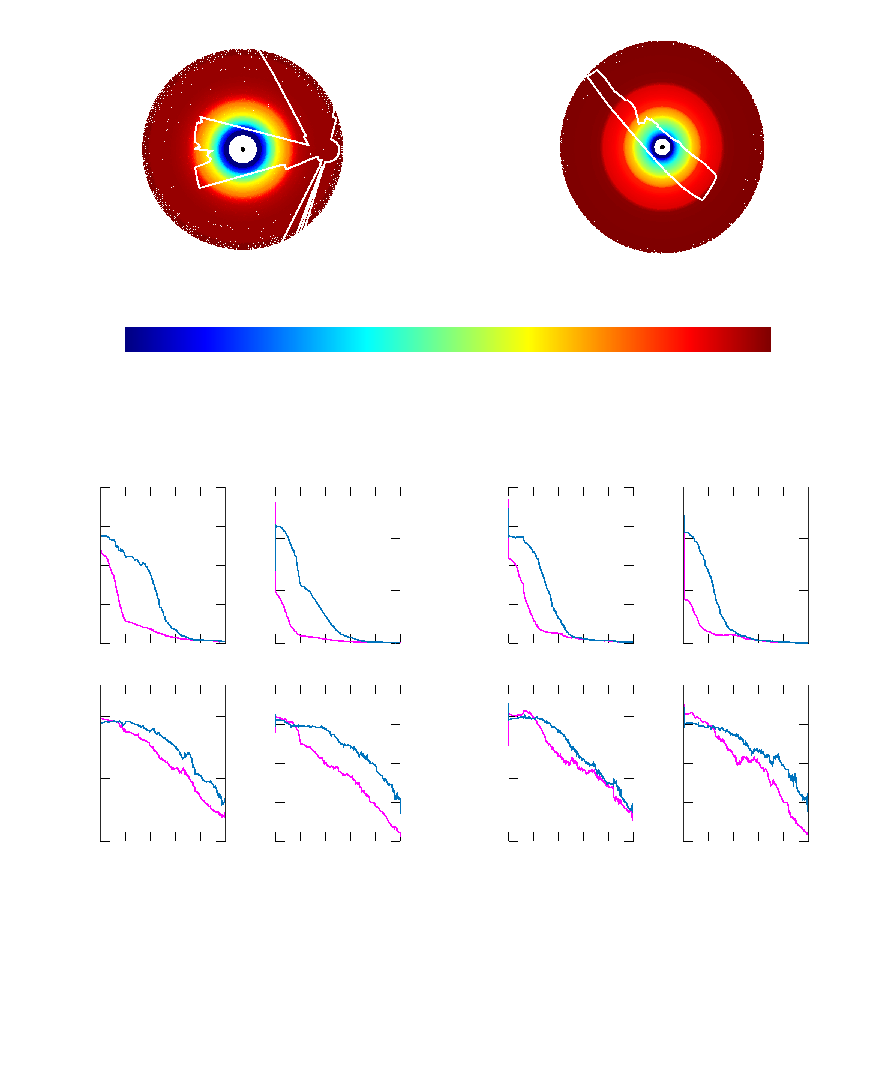
\includegraphics{./figures/parts/02/chapters/05/sections/04/max_range_test}}%
    \gplfronttext
  \end{picture}%
\endgroup

  \caption{$\sigma_R = 0.05$, da = 0.05, 10deg. db = 0.2, 0.45deg}
  \label{}
\end{figure}
